  \let\negmedspace\undefined
\let\negthickspace\undefined
\documentclass[journal]{IEEEtran}
\usepackage[a5paper, margin=10mm, onecolumn]{geometry}
\usepackage{lmodern} % Ensure lmodern is loaded for pdflatex
\usepackage{tfrupee} % Include tfrupee package

\setlength{\headheight}{1cm} % Set the height of the header box
\setlength{\headsep}{0mm}     % Set the distance between the header box and the top of the text

\usepackage{gvv-book}
\usepackage{gvv}
\usepackage{cite}
\usepackage{amsmath,amssymb,amsfonts,amsthm}
\usepackage{algorithmic}
\usepackage{graphicx}
\usepackage{textcomp}
\usepackage{xcolor}
\usepackage{txfonts}
\usepackage{listings}
\usepackage{enumitem}
\usepackage{mathtools}
\usepackage{gensymb}
\usepackage{comment}
\usepackage[breaklinks=true]{hyperref}
\usepackage{tkz-euclide} 
\usepackage{listings}                                      
\def\inputGnumericTable{}                                 
\usepackage[latin1]{inputenc}                                
\usepackage{color}                                            
\usepackage{array}                                            
\usepackage{longtable}
\usepackage{multicol}
\usepackage{calc}                                             
\usepackage{multirow}                                         
\usepackage{hhline}                                           
\usepackage{ifthen}                                           
\usepackage{lscape}
\begin{document}
	
	\bibliographystyle{IEEEtran}
	\vspace{3cm}
	
	\title{10.4.2.1.5}
	\author{EE24BTECH11063 - Y. Harsha Vardhan Reddy}
	% \maketitle
	% \newpage
	% \bigskip
	{\let\newpage\relax\maketitle}
	
	\renewcommand{\thefigure}{\theenumi}
	\renewcommand{\thetable}{\theenumi}
	\setlength{\intextsep}{10pt} % Space between text and floats
	
	
	\numberwithin{equation}{enumi}
	\numberwithin{figure}{enumi}
	\renewcommand{\thetable}{\theenumi}
	
	
\textbf{Question}:\\
Find the roots of the equation \( 100x^2-20x+1 \)
\\
\textbf{Solution: }\\
Given equation,
\begin{align}
100x^2-20x+1=0
\end{align}
We can solve the above equation using fixed point iterations. First we separate $x$, from the above equation and make an update equation of the below sort.
\begin{align}
	x = g\brak{x} \implies x_{n+1} = g\brak{x_n}
\end{align}
Applying the above update equation on our equation, we get
\begin{align}
	x_{n+1} = 	\frac{100x_n^2+1}{20}
\end{align}
Now we take an initial value $x_0$ and iterate the above update equation. But we realize that the updated values always approach infinity for any initial value. \\
Thus we will alternatively use Newton's Method for solving equations.
\begin{align}
	x_{n+1} = x_n - \frac{f\brak{x_n}}{f^{\prime}\brak{x_n}} 
\end{align}
Where we define $f\brak{x}$ as, 
\begin{align}
	f\brak{x} = 100x^2-20x+1=0 \\
	f^{\prime}\brak{x} = 200x-20 
\end{align}
Thus, the new update equation is, 
\begin{align}
	x_{n+1} = x_n - \frac{100x_n^2-20x_n+1=0}{200x_n-20 } 
\end{align}
Taking the initial guess as $x_0 = 0.05$, we can see that $x_n$ converges with x as,
\begin{align}
	x = 0.0999999 \approx 0.10
\end{align}
Alternatively, we can use the Secant method for solving equations.
\begin{align}
	x_{n+1} = x_n + f\brak{x_n}\frac{x_{n} -  x_{n-1}}{f(x_{n}) -  f(x_{n-1})}
\end{align}
Newton's method is very powerful but has the disadvantage that the derivative may sometimes be a far more difficult expression than \(f(x)\) itself and its evaluation therefore it may be more computationally expensive. The secant's method is more computationally cheap as the equation of the derivative is avoided by taking 2 starting points.\\
Alternatively, QR decomposition on Hessenberg matrix:\\
The QR decomposition method is a numerical algorithm to compute the eigenvalues of a matrix \( A \). By iteratively factorizing the matrix \( A \) into the product of an orthogonal matrix \( Q \) and an upper triangular matrix \( R \), and then recombining them in a specific order, the process converges to a diagonal matrix whose diagonal entries are the eigenvalues of \( A \).

This document adapts the QR decomposition method specifically for finding the roots of the quadratic equation \( 100x^2 - 20x + 1 = 0 \).

\section*{QR Decomposition for Quadratic Roots}
Given the quadratic equation \( 100x^2 - 20x + 1 = 0 \):
\begin{enumerate}
    \item Rewrite the equation in matrix form. For a quadratic equation \( ax^2 + bx + c = 0 \), the companion matrix is:
    \[
    A = \begin{bmatrix}
    0 & 1 \\
    -\frac{c}{a} & -\frac{b}{a}
    \end{bmatrix}.
    \]
    For \( 100x^2 - 20x + 1 = 0 \), this becomes:
    \[
    A = \begin{bmatrix}
    0 & 1 \\
    -\frac{1}{100} & -\frac{-20}{100}
    \end{bmatrix} = \begin{bmatrix}
    0 & 1 \\
    -0.01 & 0.2
    \end{bmatrix}.
    \]
    \item Perform the QR decomposition of \( A \): \( A_n = Q_n R_n \), where \( Q_n \) is an orthogonal matrix and \( R_n \) is an upper triangular matrix.
    \item Update the matrix: \( A_{n+1} = R_n Q_n \).
    \item Repeat steps 2 and 3 until \( A_n \) converges to an upper triangular matrix.
\end{enumerate}

\section*{Mathematical Description}
At the \(n\)-th iteration, let \( A_n \) be the matrix:
\[
A_n = Q_n R_n,
\]
where \( Q_n \) and \( R_n \) are obtained via the QR decomposition of \( A_n \). The matrix is updated as:
\[
A_{n+1} = R_n Q_n.
\]

\section*{Update Equation}
The update equation for the \((n+1)\)-th iteration in terms of the \(n\)-th iteration is:
\[
A_{n+1} = Q_n^T A_n Q_n,
\]
where \( Q_n \) is the orthogonal matrix from the QR decomposition of \( A_n \), and \( R_n \) is an upper triangular matrix such that \( A_n = Q_n R_n \).

\section*{Roots of the Quadratic Equation}
The eigenvalues of the companion matrix \( A \) correspond to the roots of the quadratic equation \( 100x^2 - 20x + 1 = 0 \). As the iterations progress, the diagonal elements of \( A_n \) will converge to the roots of the equation. The algorithm involves the following steps:
\begin{enumerate}
    \item Initialize \( A_0 \) as the companion matrix:
    \[
    A_0 = \begin{bmatrix}
    0 & 1 \\
    -0.01 & 0.2
    \end{bmatrix}.
    \]
    \item Perform the QR decomposition of \( A_n \):
    \[
    A_n = Q_n R_n,
    \]
    where \( Q_n \) is orthogonal and \( R_n \) is upper triangular.
    \item Compute \( A_{n+1} \) using the update equation:
    \[
    A_{n+1} = R_n Q_n.
    \]
    \item Repeat until \( A_n \) converges to an upper triangular matrix. The diagonal elements of this matrix are the eigenvalues, which correspond to the roots of the quadratic equation.
\end{enumerate}

\section*{Conclusion}
The QR decomposition method applied to the companion matrix of \( 100x^2 - 20x + 1 = 0 \) numerically finds the roots of the equation. The iterative process demonstrates how eigenvalue computation can be used effectively to determine the roots without relying on direct formulas.



The code which computes this gives equal roots as "0.1000 + 0.0000 j"
\newline\newline
	\begin{figure}[h!]
		\centering
		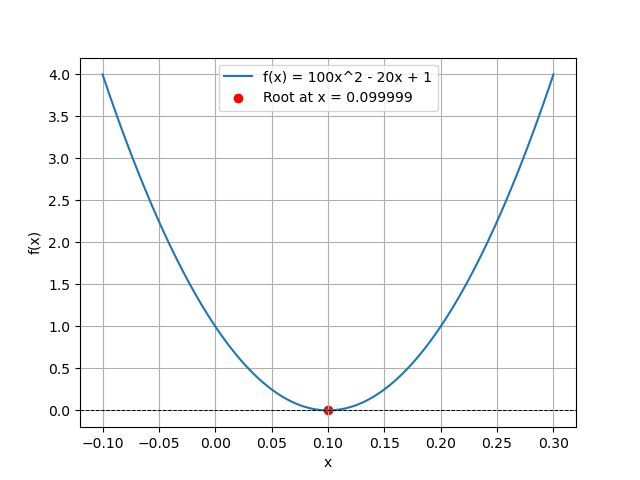
\includegraphics[width=\columnwidth]{figs/Figure_1.png}
		\caption{Solution of the given function}
		\label{stemplot}
	\end{figure}


\end{document}  
